
\subsection*{Descubriment de Reflexió total en l'any 1841}
\addcontentsline{toc}{subsection}{Descubriment de Reflexió total en l'any 1841}

La reflexió total és el fenomen físic que es produeix quan un raig de llum incideix amb un angle superior a l'angle crític en una superfície transparent d'índex de refracció alt. Per angles d'incidència majors o iguals a l'angle crític, tota l'energia és reflectida cap al medi incident.
S'utilitza en la fibra òptica, fent que l'índex de refracció de l'interior sigui més gran que l'aire. D'aquesta manera un raig que emetem des del principi no surt del fil fins que no es talla. 

\begin{figure}[h!]
    \centering
    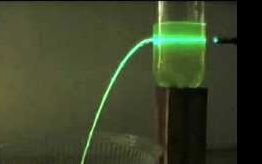
\includegraphics[width=80mm]{refluxiototal.png}
    \caption{Teoría reflexió total}
\end{figure}


\subsection*{Generació de la fibra òptica}
\addcontentsline{toc}{subsection}{Generació de la fibra òptica}

\subsubsection*{Capa física de fibra:}

\begin{itemize}
    \item 1887: El científic britànic Charles va fabricar fibra de vidre per primera vegada.
    \item 1938: Dues empreses nord-america i japonés van poder fabricar dibra de vidres més llargues.
    \item 1956: un estudiant de la Universitat de Michigan va utilitzar un tub de vidre de baix índex de refracció i el va fondre en una vareta de vidre d'alt índex de refracció, creant la primera fibra òptica revestida de vidre. 

\end{itemize}

\subsubsection*{Defeneix utilitat de la fibra:}

\begin{itemize}
    \item 1966: Físic Charles Kuen Kao es van posar les bases de les comunicacions de fibra òptica.
    \item 1971: Es llança la primera fibra òptica d'un quilòmetre de llargada.
    \item 1981: Es comença el sistema de comunicació de fibra òptica.
\end{itemize}



\subsection*{La idea de Li-Fi}
\addcontentsline{toc}{subsection}{La idea de Li-Fi}

La tecnologia Li-Fi va ser proposada per primera vegada pel professor Harald Haas de la Universitat d'Edimburg durant una conferència TED Talk al juliol de 2011. En aquesta presentació, el professor Haas va descriure la possibilitat d'utilitzar la llum LED per a transmetre dades de manera inalàmbrica, una idea que va conduir al desenvolupament de la tecnologia Li-Fi.



